\documentclass[a4paper,12pt]{article}
\usepackage[italian]{babel}
\usepackage{graphicx}

%opening
\title{\textbf{Studio di un modello di influenza culturale}}
\author{Jacopo Baldassarri, Andrea Blasco, Elisa Omodei}

\begin{document}

\maketitle

\begin{abstract}
Studiamo un modello di evoluzione culturale alla Axelrod (1997) in cui l'interazione tra gli agenti avviene all'interno di una rete sociale di amicizie. Gli agenti sono disposti su di un reticolo di tipo ``torus'' e formano  connessioni tra di loro tramite un modello che con unico parametro ci consente di catturare diverse tipologie di reti sociali. Queste si differenziano principalmente per il grado di dipendenza delle amicizie dalla posizione degli agenti nel reticolo; quando la dipendenza \`{e} massima studiamo un rete locale, per valori intermedi abbiamo uno \textit{small world} ed infine un \textit{random network} quando c'\`e indipendenza.    \\   
In generale troviamo che l'evoluzione culturale \`{e} soggetta ad una transizione di fase, ovvero esiste un valore critico di disordine iniziale del sistema al di sotto del quale l'eterogeneit\`{a} dei tratti culturali non viene preservata dall'interazione sociale.\\
Sorprendentemente, in presenza di reti con un basso grado di dipendenza dal reticolo, la transizione di fase sembra avvenire in maniera continua invece che discontinua come documentato nella maggior parte degli studi precedenti. 
%Questo avviene, molto probabilmente, a causa della presenza crescente di connessioni non reciproche
\end{abstract}

\clearpage
\section{Introduzione}
La domanda con cui esordisce R.~Axelrod nel suo articolo del 1997 \cite{Axelrod} \`{e}: \textquotedblleft If people tend to become 
more alike in their beliefs, attitudes, and behavior when they interact, why do not all such differences eventually disappear?\textquotedblright .
\\Il modello da lui proposto parte dal fatto che le persone diventano pi\`{u} simili quando interagiscono, ma spiega anche perch\`{e}
questa tendenza alla convergenza si ferma prima di arrivare ad una completa convergenza.
\\Il termine pi\`{u} generico per denotare le cose in cui le persone si influenzano a vicenda \`{e} \textit{cultura}.
Dunque questo termine verr\`{a} d'ora in poi utilizzato per indicare l'insieme di caratteristiche individuali che sono soggette all'influenza sociale.
\\Il modello di influenza sociale proposto astrae il principio fondamentale che il trasferimento di idee avviene pi\`{u} frequentemente
tra individui che sono gi\`{a} simili in alcuni aspetti, per affermare che la comunicazione \`{e} pi\`{u} efficace tra persone simili:
la probabilit\`{a} che un tratto culturale venga trasmesso da un individuo (o un gruppo) ad un altro dipende da quante altre caratteristiche
hanno gi\`{a} in comune.
\\Si parte dall'assunzione che la cultura deve soddisfare due semplici principi: 
\begin{itemize}
\item \`{e} pi\`{u} probabile che le persone interagiscano con altre persone con cui hanno gi\`{a} delle caratteristiche in comune,
\item le interazioni tra due persone tendono ad aumentare il numero di caratteristiche in comune.
\end{itemize}
Il modello assume che la cultura di un individuo si possa descrivere in termini di caratteristiche come la lingua, la religione,
l'abbigliamento, ecc. La cultura \`{e} dunque descritta come un insieme di caratteristiche. 
Per ogni caratteristica c'\`{e} un insieme di tratti, che sono i valori alternativi che una caratteristica pu\`{o} assumere.
Due individui hanno la stessa cultura se hanno gli stessi tratti per ognuna delle caratteristiche. 
Questa formulazione permette di definire il grado di somiglianza culturale tra due individui come la percentuale di caratteristiche che hanno lo stesso tratto.

\clearpage
\section{Il Modello di Axelrod}
Il modello standard di Axelrod \`{e} definito su un reticolo quadrato di dimensione lineare \textit{L} con condizioni periodiche al contorno. 
Ogni sito \textit{i} \`{e} caratterizzato da un vettore \textit{F}-dimensionale di variabili $\sigma_f(i)$ che definiscono le caratteristiche culturali degli individui di quel sito.
Ogni caratteristica $f=1,\dots,F$ di ogni sito \`{e} inizialmente presa da una distribuzione casuale uniforme di interi compresi tra 0 e $q-1$: $\sigma_f = 0,1,\dots,q-1$.
Il parametro \textit{q} \`{e} una misura della variet\`{a} culturale (disordine) iniziale nel sistema.
Ad ogni passo temporale, una coppia di siti vicini \textit{i} e \textit{j} viene selezionata in modo casuale e viene misurata la loro somiglianza culturale, cio\`{e} la quantit\`{a}:
\begin{equation}
 \omega_{i,j} = \frac{1}{F} \sum_{f=1}^F \delta_{\sigma_f(i) \sigma_f(j)}
\end{equation}
dove $\delta_{i,j}$ \`{e} la delta di Kronecker.
Con probabilit\`{a} pari a $\omega_{i,j}$ avviene l'interazione: una a caso tra le caratteristiche per cui i tratti sono diversi 
$[ \sigma_f(i) \neq \sigma_f(j) ]$ viene selezionata e il tratto di \textit{j} viene posto uguale a quello di \textit{i}.
Con probabilit\`{a} $1-\omega_{i,j}$ non succede niente.
Uno \textit{sweep} di tutto il reticolo, cio\`{e} $L^2$ passi temporali, definisce l'unit\`{a} temporale.
Se tutte le caratteristiche sono uguali su un legame o se sono tutte diverse, nessun cambiamento pu\`{o} pi\`{u} avvenire sul tale legame.
Una tale configurazione \`{e} detta \textit{stato assorbente}. La dinamica si ferma quando un tale stato \`{e} raggiunto.
\\L'evoluzione dinamica \`{e} caratterizzata dalla competizione tra il disordine della configurazione iniziale e la spinta all'ordine
dovuta alle interazioni sociali locali. 
Quando $q$ \`{e} piccolo lo stato iniziale \`{e} quasi completamente uniforme, mentre quando $q$ \`{e} grande quasi tutti i siti
hanno caratteristiche $\sigma_f(i)$ completamente diverse dai propri vicini. Nei due casi ci aspettiamo che il sistema converga ad
uno stato uniforme o altamente fragmentato in cui dominano le interazioni o il disordine, rispettivamente.
Castellano \textit{et al.} \cite{Castellano} hanno studiato come queste due situazioni limite sono connesse al variare di $q$
e hanno trovato che per $F>2$ avviene una transizione netta ad un certo valore critico $q_c$ di $q$ caratterizzata da un
improvviso calo del parametro d'ordine $<S_{max}>/L^2$, transizione che diventa sempre pi\`{u} ripida all'aumentare di $L$.
Ci\`{o} mette in evidenza una transizione tra una fase culturalmente polarizzata per $q<q_c$, dove una delle regioni culturali ha
le dimensioni dell'ordine di tutto il sistema, e una fase culturalmente frammentata, dove tutte le regioni culturali hanno dimensione finita.
La situazione \`{e} invece diversa per $F=2$, per cui la frazione occupata da $<S_{max}>/L^2$ diminuisce con continuit\`{a} all'aumentare di $q$.
Castellano ha inoltre trovato che la distribuzione delle dimensioni delle regioni culturali $P_L(s,q)$ per valori di $q$ attorno alla transizione
segue una legge di potenza $P_L(s,q) = s^{-\tau}$.

\subsection{Risultati con Interazione Locale}
Come \`e chiaro dalla descrizione precedente, il modello di Axelrod assume implicitamente che l'interazione avvenga esclusivamente in maniera locale ovvero che la dipendenza delle connessioni dalla vicinanza degli agenti sul reticolo \`e massima. 	\\	 
Partendo da questo caso particolare, abbiamo dunque iniziato il nostro studio effettuando delle simulazioni numeriche per il caso $F=3$ e $L=20$.
Abbiamo scelto il caso $F=3$ per poter avere una buona visualizzazione grafica del modello. Infatti in questo modo ci \`{e} possibile associare ad ogni caratteristica una componente RGB e possiamo dunque rappresentare ogni cultura con un colore attraverso una corrispondenza biunivoca (vedi Figura \ref{fig:colors}).
\begin{figure}[!ht]
\centering 
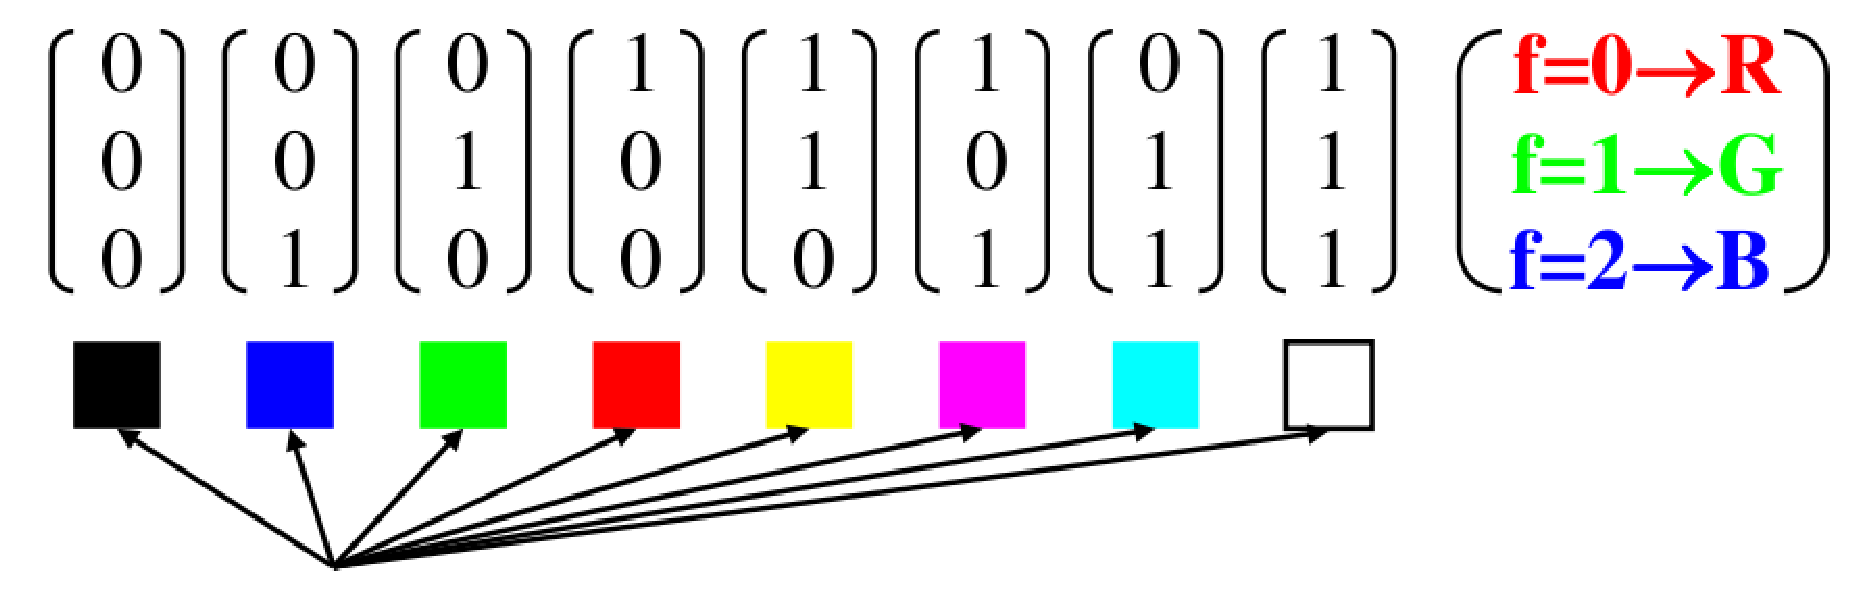
\includegraphics[width=0.75\textwidth]{colors.eps}
\caption{Esempio di corrispondenza tra tratti culturali e colori RGB	\label{fig:colors}}
\end{figure}
\\ \\La Figura \ref{transiz_ret} mostra la transizione, ovvero come varia il parametro d'ordine $<S_{\max}>/L^2$ al variare di $q$. 
Possiamo osservare una transizione abbastanza netta attorno a $q = q_c \simeq 12$. I valori sono mediati su dieci realizzazioni, 
per cui \`{e} riportata anche la varianza.
La Figura \ref{cum_distr_size_ret} mostra la distribuzione, in scala logaritmica, delle dimensioni delle regioni culturali 
per $q_c = 12$. Possiamo osservare che essa sembra seguire effettivamente una legge di potenza con esponente $\tau \simeq 2$.
\begin{figure}
\begin{center}
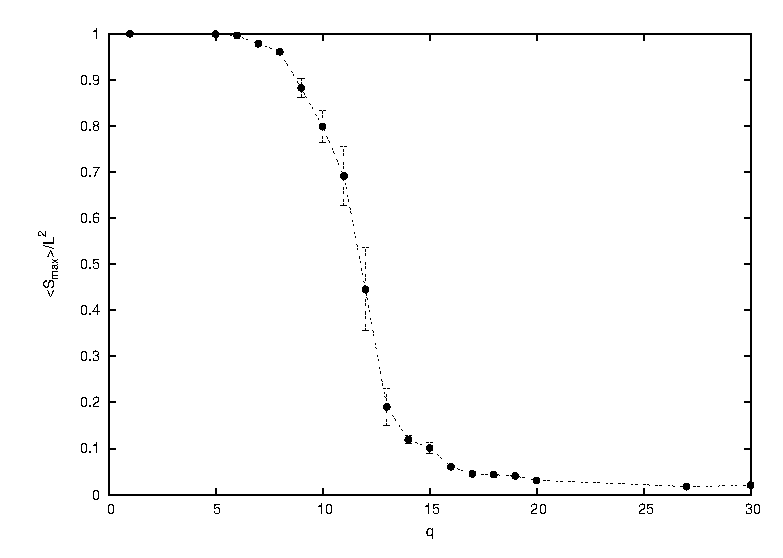
\includegraphics[width=0.7\textwidth]{transizione_ret.eps}
\end{center}
\caption{Transizione tra una fase culturalmente polarizzata e una fase culturalmente fragmentata al variare di $q$ nel caso del modello di Axelrod originale, ovvero su reticolo con quattro vicini. La transizione \`{e} studiata attraverso il parametro d'ordine $<S_{\max}>/L^2$. I risultati ottenuti sono mediati su dieci realizzazioni ed \`{e} riportata dunque anche la varianza. }
\label{transiz_ret} 
\end{figure}

\begin{figure}[!ht]
\begin{center}
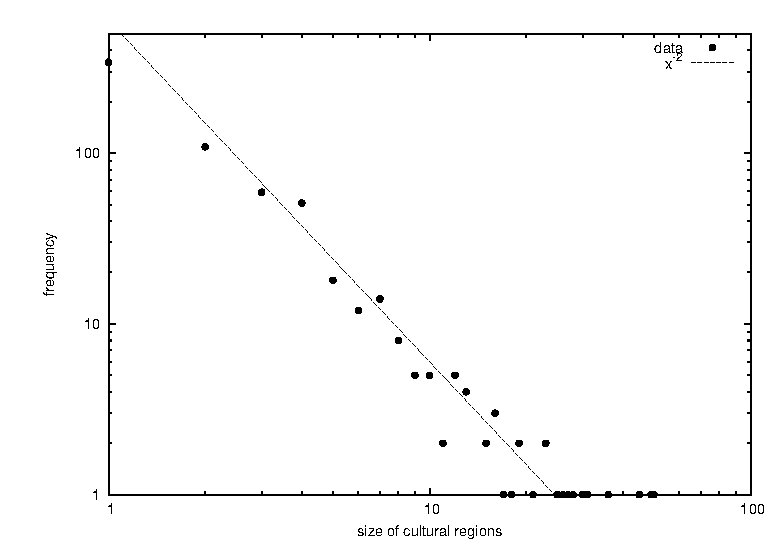
\includegraphics[width=0.7\textwidth]{cum_distr_size_ret.eps}
\end{center}
\caption{Distribuzione delle dimensioni delle regioni culturali per $q = q_c$, in scala logaritmica per entrambi gli assi, nel caso del modello di Axelrod originale, ovvero su reticolo con quattro vicini. I risultati ottenuti sono basati su dieci realizzazioni.}
\label{cum_distr_size_ret}
\end{figure}

\begin{figure}[!ht]
\begin{center}
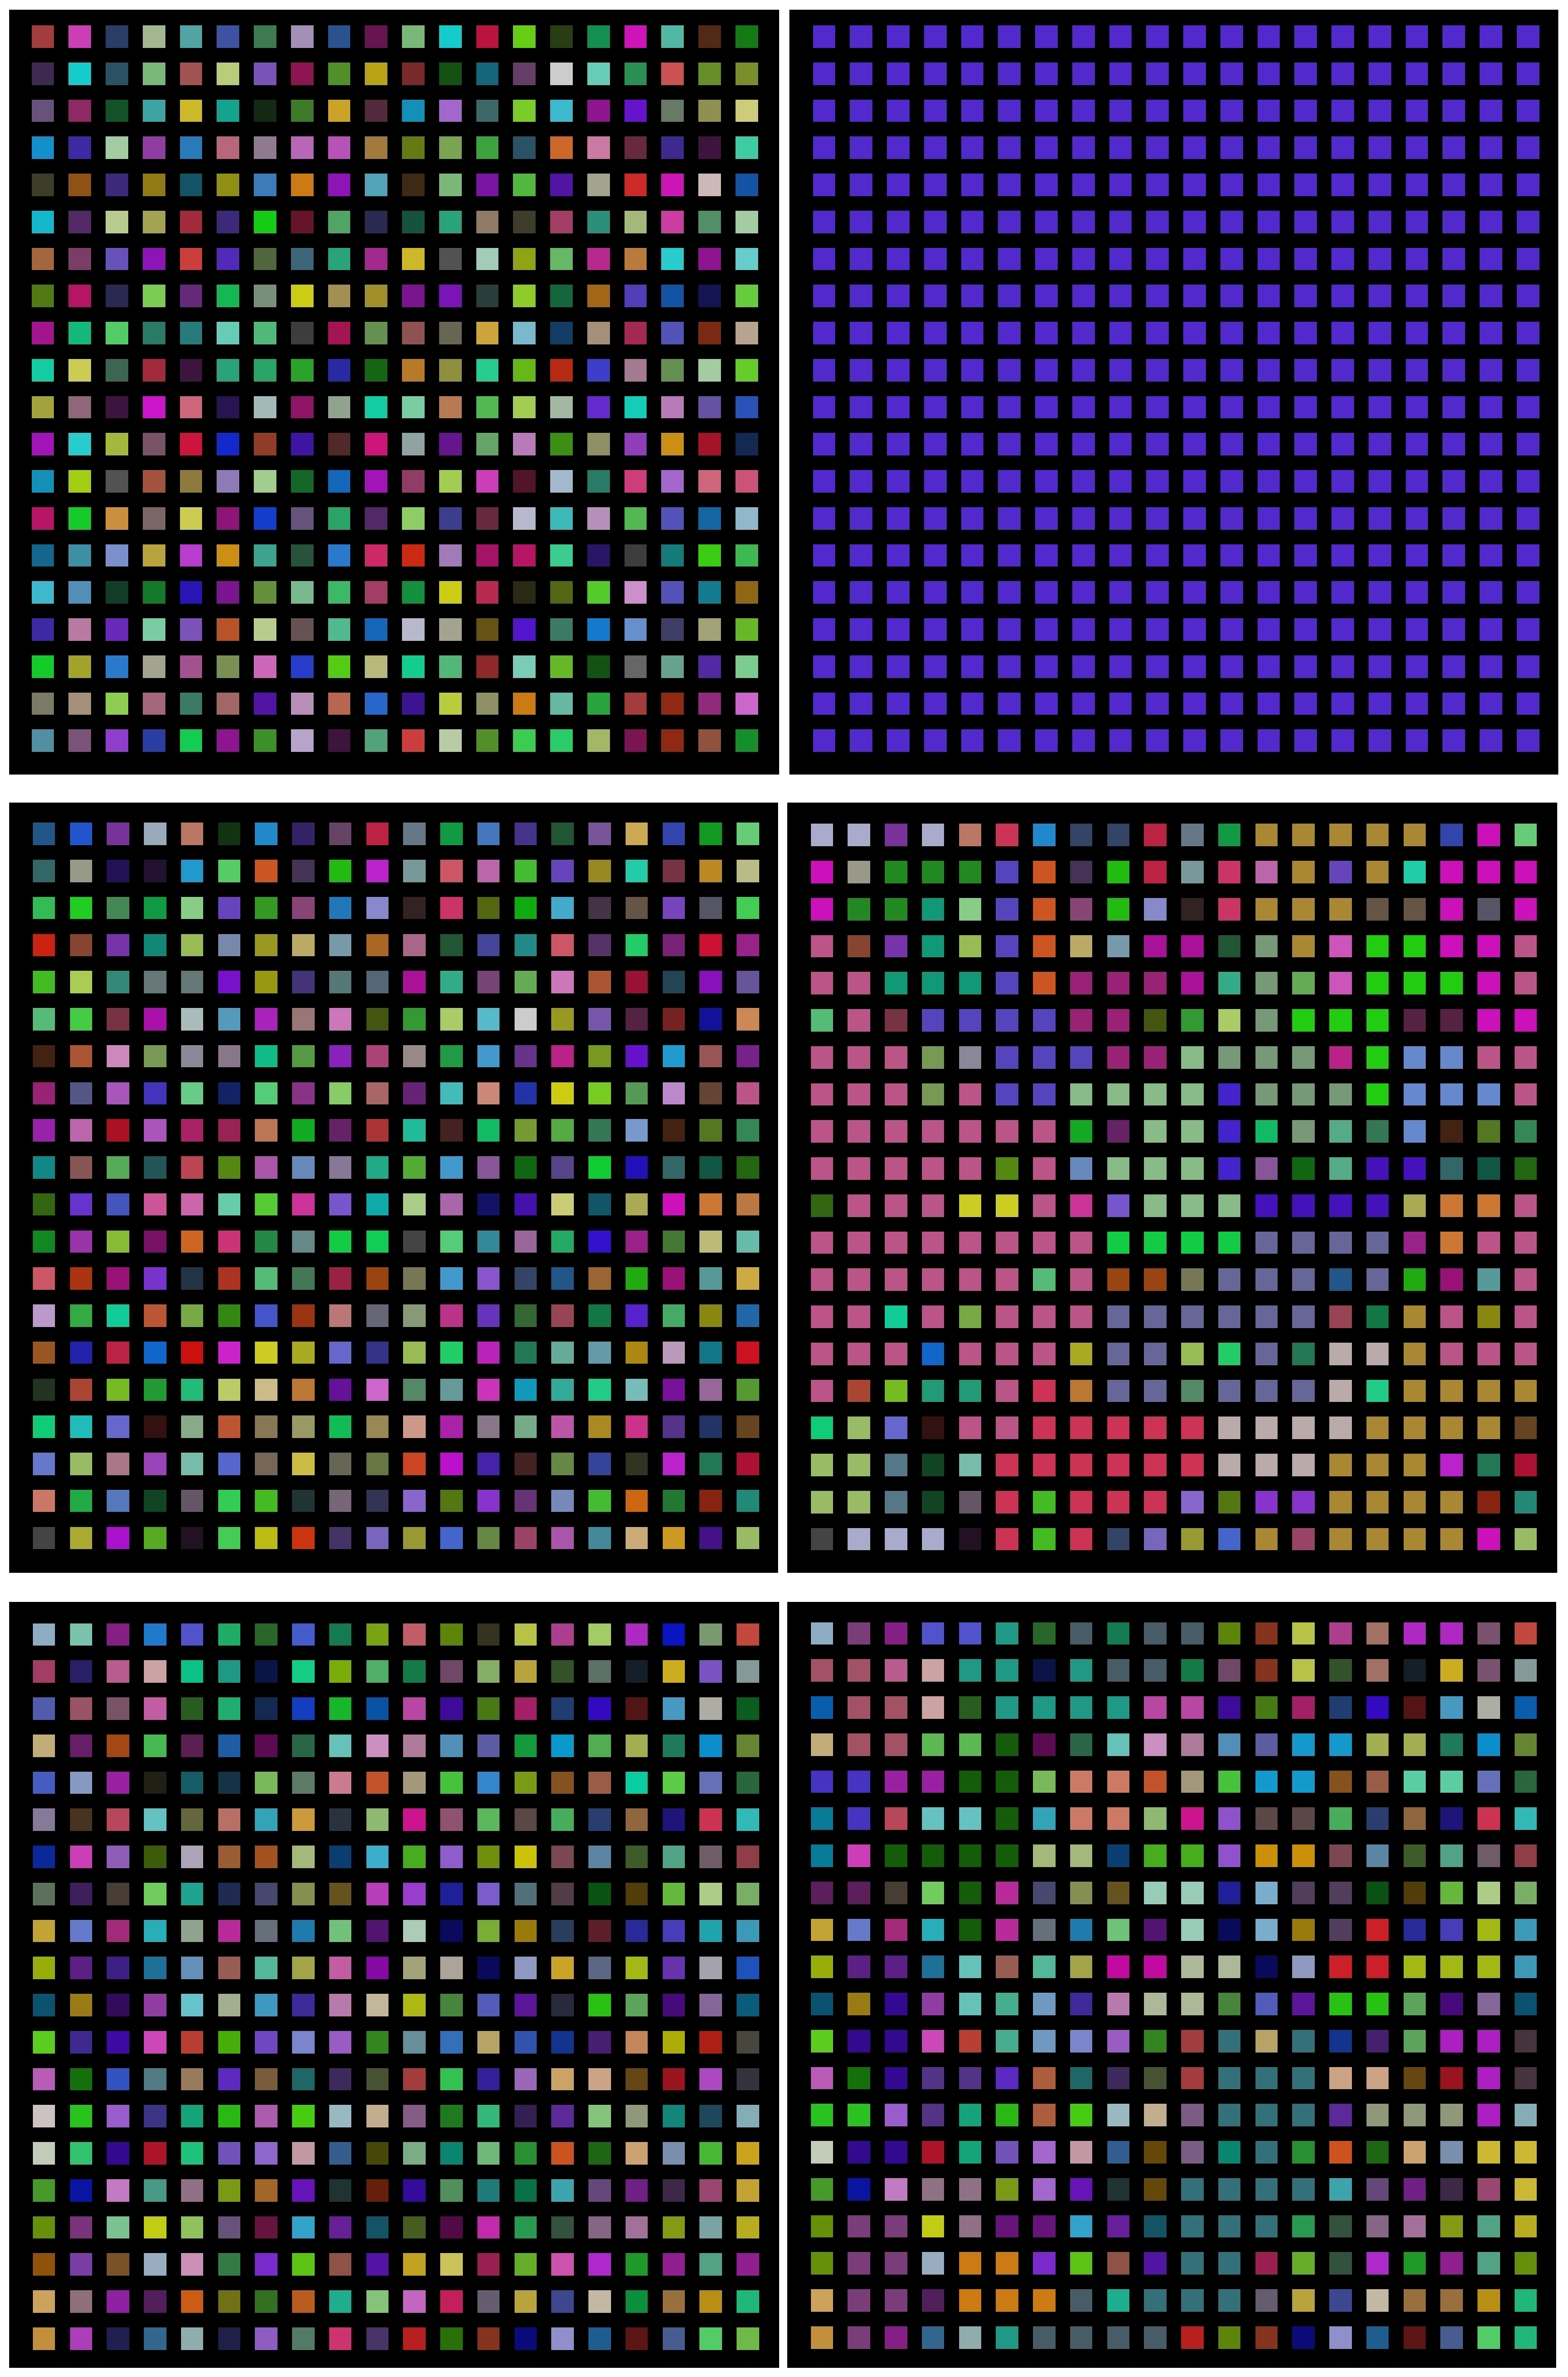
\includegraphics[width=0.85\textwidth]{axelrod.eps}
\end{center}
\caption{Fotografia della rete con interazione locale all'istante inziale (sinistra) e all'istante finale (destra) della dinamica, per diversi valori di \textit{q}. Le prime due figure si riferiscono al caso $q<q_c$, le seconde due al caso $q = q_c$ e le ultime due al caso $q>q_c$.}
\label{axelrod}
\end{figure}

\clearpage

\section{L'Evoluzione Culturale su Reti Sociali}
Abbiamo poi deciso di estendere il modello standard di Axelrod a diversi tipi di reti sociali. In particolare abbiamo studiato la medesima dinamica evolutiva della cultura applicata al modello di rete proposto da Kleinberg in \cite{Kleinberg}.
\\ \\Consideriamo dunque $N$ nodi o agenti identificati da un insieme di punti su di un toro di dimensioni $L \times L$, ${(i,j) : i \in {1,2,\dots,L}, j \in {1,2,\dots,L}}$ e definiamo la distanza tra due nodi $(i,j)$ e $(k,l)$ come 
\begin{center}
$d((i,j),(k,l)) = \sqrt{(i-k)^2+(j-l)^2}$.
\end{center}
Ogni nodo avr\`{a} lo stesso numero quattro di link uscenti; ciascun link diretto dal nodo \textit{u} al nodo \textit{v} viene creato in modo 
casuale con probabilit\`{a} proporzionale a $[d(u,v)]^{-\delta}$, dove $\delta\in [0,\infty]$ \`{e} un parametro che cattura l'importanza della vicinanza geografica nel reticolo. \\
Quando $\delta = 0$ la distanza tra due nodi non influenza la probabilit\`a di stabilire una connessione e teoricamente si ottiene una distribuzione uniforme dei contatti a lungo raggio. 
Al crescere di $\delta$ invece i contatti a lungo raggio diventano sempre pi\`{u} clusterizzati nelle vicinanze del nodo stesso. In questo modo il caso visto in precedenza di una rete locale si ottiene quando $\delta = \infty$.
%Adesso il modello di creazione delle connessioni ha una chiara interpretazione geografica, rappresenta infatti un parametro strutturale che misura quanto ampiamente \`{e} interconnessa la societ\`{a} dei nodi.\\
\\ \\Inoltre \`e utile rimarcare che a causa della direzionalit\`a delle connessioni, quando $\delta<\infty$, si possono creare amicizie non necessariamente reciproche. Mentre questo ovviamente non \`e possibile quando le connessioni sono esclusivamente locali e quindi un agente conosce solo i suoi vicini e viceversa, nel caso generale \`e possibile che un agente venga influenzato dai suoi amici diretti ma non viceversa. Per esempio si verifica la seguente situazione in cui un agente vuole imitare i tratti di un suo amico ma quest'ultimo \`e invece influenzato da altri agenti che considera pi\`u importanti rispetto al primo. \\	
Dalla direzionalit\`a dei link  deriva anche che il sistema pu\`{o} non raggiungere mai uno stato \textit{completamente} assorbente. Questo \`{e} dovuto, ad esempio, alle situazioni in cui un agente \textit{u} viene alternativamente influenzato da due suoi vicini che hanno in comune tra loro e con l'agente \textit{u} due caratteristiche su tre. In questo caso il sistema converge verso un insieme di alterne configurazioni culturali molto simili che si avvicendano in maniera oscillatoria.
% ma se l'agente $i$ ha dei link uscenti verso questi altri due agenti ma non viceversa, allora i due agenti continueranno ad influenzare l'agente $i$, ma esso non potr\`{a} influenzare loro.
\\Si osserva tuttavia che dopo un certo numero di step temporali tutte le quantit\`{a} interessanti del sistema rimangono costanti in media e il sistema \`{e} dunque termalizzato. In questo caso quindi la dinamica viene fermata dopo un numero di step temporali pari al quadrato del numero di agenti, tempo che abbiamo visto essere pi\`{u} che sufficiente per raggiungere la termalizzazione.

\subsection{Risultati}
Come evidente dalla Figura \ref{transiz}, al diminuire di $\delta$ la transizione dalla fase culturalmente polarizzata a quella culturalmente fragmentata avviene in modo sempre meno netto. In particolare,  mentre con una rete locale, $\delta = \infty$, sembra esserci una discontinuit\`a attorno al valore critico,  questo non avviene per il caso del random network, $\delta=0$, in cui sono invece possibili diversi stati intermedi in cui gli effetti dell'evoluzione verso una cultura dominante sembrano dimuire quasi linearmente al crescere del parametro di disordine iniziale. \\
La pendenza della curva di transizione dipende dunque dalla geografia del network: pi\`{u} globalizzata \`{e} la rete, maggiore \`{e} il numero di possibili tratti necessari perch\`{e} vi sia una netta fragmentazione culturale. \\
\\Inoltre anche in questo caso otteniamo delle leggi di potenza per la distribuzione delle dimensioni delle regioni culturali attorno a $q_c$, con esponente $\tau$ che diminuisce al diminuire di $\delta$ (Figura \ref{cum_distr_size}).

\begin{figure}[!ht]
\begin{center}
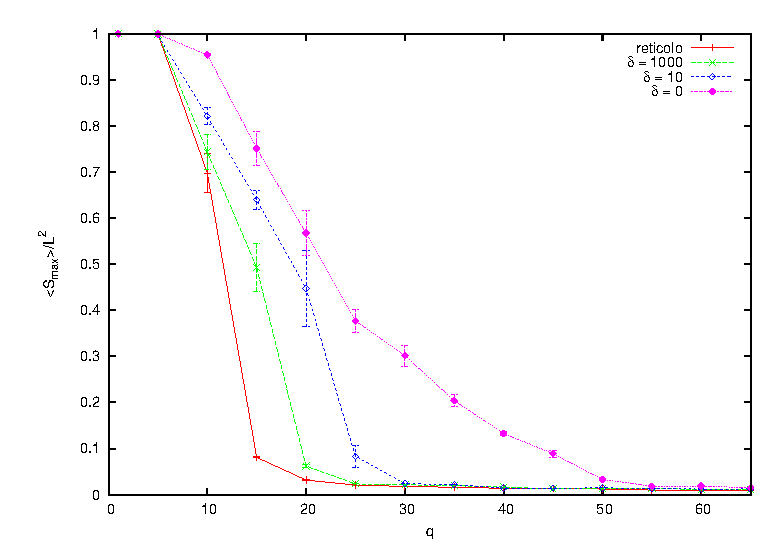
\includegraphics[width=0.8\textwidth]{transizione.eps}
\end{center}
\caption{Transizione tra una fase culturalmente polarizzata e una fase culturalmente fragmentata al variare di $q$, per diversi valori del parametro $\delta$. La transizione \`{e} studiata attraverso il parametro d'ordine $<S_{max}>/L^2$. I risultati ottenuti sono mediati su dieci realizzazioni ed \`{e} riportata dunque anche la varianza.}
\label{transiz}
\end{figure}

\begin{figure}[!ht]
\begin{center}
\includegraphics[width=\textwidth]{cum_distr_size_qCritico.eps}
\end{center}
\caption{Distribuzione delle dimensioni delle regioni culturali per $q = q_c$, in scala logaritmica per entrambi gli assi, per diversi valori del parametro $\delta$. I risultati ottenuti sono basati su dieci realizzazioni.}
\label{cum_distr_size}
\end{figure}

\clearpage
\section{Software}
Il progetto \`e stato implementato utilizzando il linguaggio C++, con l'utilizzo delle librerie fltk sotto ambiente Linux. Sono stati
utilizzati gli editor Kate e Gedit per la scrittura del codice, il programma Gnuplot per la realizzazione delle figure e l'ambiente Kile per
la stesura della relazione.\\
Abbiamo deciso 
di suddividere il codice in due parti distinte, una parte testuale, in cui non vi \`e nessun tipo di visualizzazione del modello, che ci 
permette di fare delle simulazioni molto velocemente, ed una parte grafica nel quale viene visualizzata una vista del modello e dove \`e 
possibile modificare i vari parametri di simulazione a run time.
\subsection{Grafica}
La parte grafica \`e stata realizzata mediante l'utilizzo delle librerie fltk, \`e stato creato un file elanja-fltk.cxx con l'inizializzazione di tutti 
gli elementi grafici della nostra interfaccia, quali slider, bottoni per il controllo di sequenza, ecc., e delle classi per l'implementazione
del  nostro modello.\\
Nella classe simulationGrid.cpp viene realizzata la parte grafica, in cui vengono disegnati tutti gli agenti e i link fra di essi;
\`e la classe che si occupa anche della reinizializzazione grafica nel caso in cui vengano modificati i parametri del modello.\\
Il compito della realizzazione vera e propria del modello \`e affidata alla classe model.cpp nella quale vengono inizializzate tutte le strutture 
dati necessarie alla simulazione: mediante l'utilizzo di malloc per l'allocazione della memoria, viene riservato spazio per le matrici nel quale 
andranno ad essere inseriti i dati degli agenti, delle loro connessioni e delle loro caratteristiche culturali. Inoltre la classe si occupa dell'aggiornamento delle matrici, calcolando ad 
ogni passo di iterazione gli opportuni valori delle caratteristiche culturali che vengono inseriti nelle strutture dati.\\
Vi \`e inoltre una classe widgetWindow.cpp che si occupa di creare e di aggiungere all'interfaccia grafica delle finestre di statistiche sulle
quali vengono visualizzati dei valori interessanti del modello, che vengono monitorati a run time durante la simulazione.\\
Abbiamo inoltre una superclasse glStats.cpp che rappresenta una generica statistica da visualizzare in una delle sotto-finestre, nella quale 
vengono impostati tutti i parametri di visualizzazione.\\
Sono invece le tre sottoclassi cultureStats.cpp, maxRegionStats.cpp e regionCountStats.cpp che implementano la visualizzazione delle statistiche del
modello che vengono disegnate a run time nelle sotto-finestre. 
In particolare, cultureStats.cpp visualizza la distribuzione regioni culturali, maxRegionStats.cpp visualizza il numero di agenti appartenenti alla regione pi\`{u} grande ad ogni istante di tempo, regionCountStats.cpp visualizza il numero di regioni culturali presenti nel sistema ad ogni istante di tempo.\\
Abbiamo infine la classe gui\_controls.cpp, in cui sono realizzate tutte le funzioni per gli slider dell'interfaccia grafica e per i pulsanti di 
controllo  di sequenza, quali play, pause e stop.\\
Nell'interfaccia grafica ogni agente viene rappresentato da un quadratino e il colore di ogni quadratino \`{e} dato da una 
combinazione dei valori dei tre tratti culturali dell'agente, ciascuno dei quali viene mappato in una componente RGB mediante una trasformazione lineare.

\subsection{Testuale}
Nella parte testuale ovviamente le classi che abbiamo realizzato sono notevolmente ridotte, infatti non sono pi\`u necessarie tutte le parti
di visualizzazione del modello e delle statistiche.\\
Abbiamo in questa parte solo due classi, la classe elanja.cpp che \`e il main del progetto testuale e che si occupa di eseguire i passi di 
simulazione e di stampare delle statistiche in dei file specificati cos\`i che queste possano essere elaborate in un secondo momento. Essa si 
occupa anche di inizializzare i parametri del modello, o in base a dei parametri di default, contenuti nel file const.h, oppure in base ai
parametri che l'utente fornisce al momento dell'invocazione dell'eseguibile del progetto da terminale. Infatti in questo frangente \`e 
possibile specificare al momento dell'esecuzione quali sono i parametri con i quali fare le simulazioni, mentre nella sezione grafica questo 
non \`e supportato, dato che \`e possibile farlo a run time mediante l'interfaccia grafica.

\begin{figure}[!ht]
\begin{center}
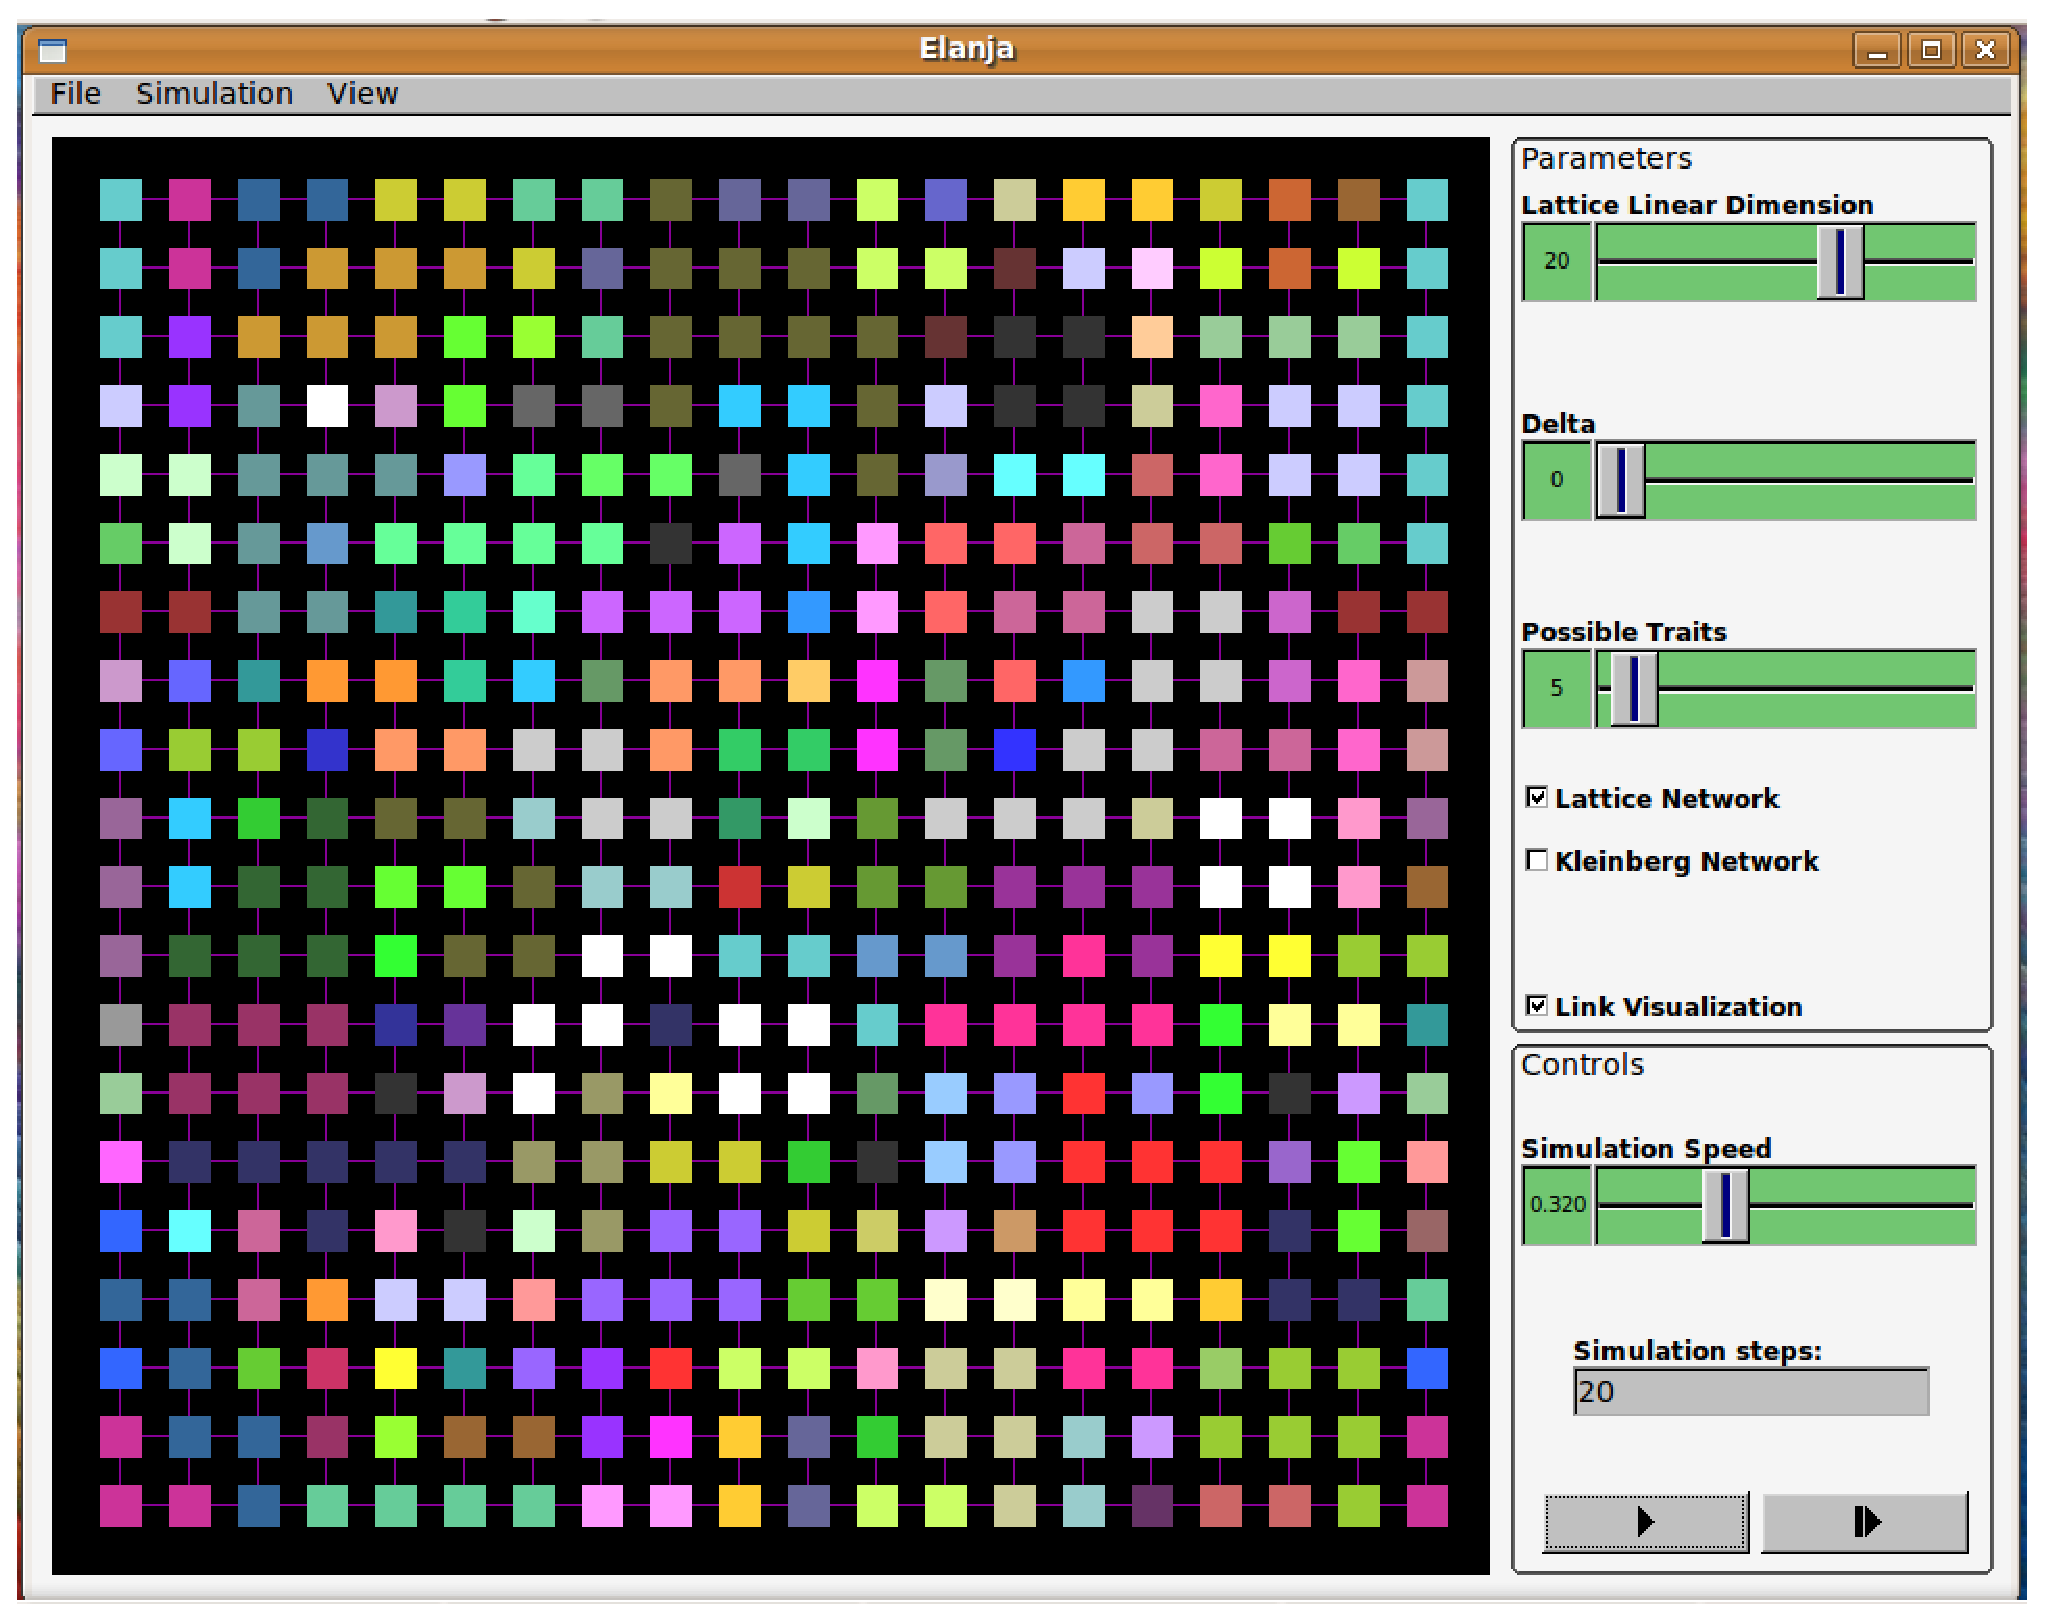
\includegraphics[width=\textwidth]{elanja.eps}
\end{center}
\caption{Interfaccia grafica del sistema}
\end{figure}

\clearpage
\begin{thebibliography}{10}
\normalsize
 \bibitem{Axelrod} R.~Axelrod, \textit{The Dissemination of Culture}, Journal of Conflict Resolution, 41, 203 (1997)
 \bibitem{Castellano} C.~Castellano, M.~Marsili and A.~Vespignani, \textit{Nonequilibrium phase transition in a model for social influence}, Phys.~Rev.~Lett. 85, (2000)
 \bibitem{Klemm} K.~Klemm, V.~M.~Eguiluz, R.~Toral and M.~San~Miguel, \textit{Nonequilibrium transitions in complex networks: a model of social interaction}, Phys.~Rev.~E 67 (2003)
 \bibitem{Kleinberg} J.~Kleinberg, \textit{The Small-World Phenomenon: An Algorithmic Perspective}, Proceedings of the thirty-second annual ACM symposium on Theory of computing (2000)
 \bibitem{Barabasi} R.~Albert and A.-L.~Barabasi, \textit{Statistical mechanics of complex networks}, Rev.~Mod.~Phys. 74 (2002)
 \bibitem{Jackson} M.~O.~Jackson, \textit{Social and Economic Networks}, Princeton University Press (2008) 
\end{thebibliography}

\end{document}
